%%%%%%%%%%%%%%%%%%%%%%%%%%%%%%%%%%%%%%%%%%%%
\section{Selection of Observing Fields [TBD]\label{sec:RasterField}}

In this section, we describe the preparation of target objects for the on-sky commissioning and the performance verification. We suppose three cases of target fields, 1. a field with many bright stars such as an open cluster for the raster scan, 2. a field with a sufficient number of bright stars such as an SDSS field at high galactic latitude for the throughput measurement and the verification of the flux calibration, 3. a field with faint galaxies and stars for the verification of long exposure. We briefly describe each case and possible candidate targets below.

\subsection{Open Clusters as the Raster Targets}
For the raster scan process, targets should be sufficiently bright and point sources for the accurate evaluation in the analysis. In addition, they should cover the entire PFS FoV and the number density should be matched to the PFS fiber density. Open clusters with sufficient bright member stars in the Galaxy are plausible targets for the raster scan. 

The candidate open clusters are selected from DAML02 catalogue (Dias et al. 2002, A\&A, 389, 871), which includes information on fundamental parameters (distance, apparent diameter, proper motion, age, reddening, metallicity, and so on) of $\sim2000$ open clusters.  Figure \ref{fig:RasterFieldMap1} and Figure \ref{fig:RasterFieldMap2} show the spatial distribution of the open clusters with the apparent diameter ($d$ [deg.]) of $>30$. There exist $\sim130$, $\sim50$, $\sim30$ open clusters with the apparent diameter of $30<d<60$, $60<d<120$, and $d>120$, respectively. The typical number of member stars is $\sim1000$. 

\begin{figure}[!ht]
\begin{center}
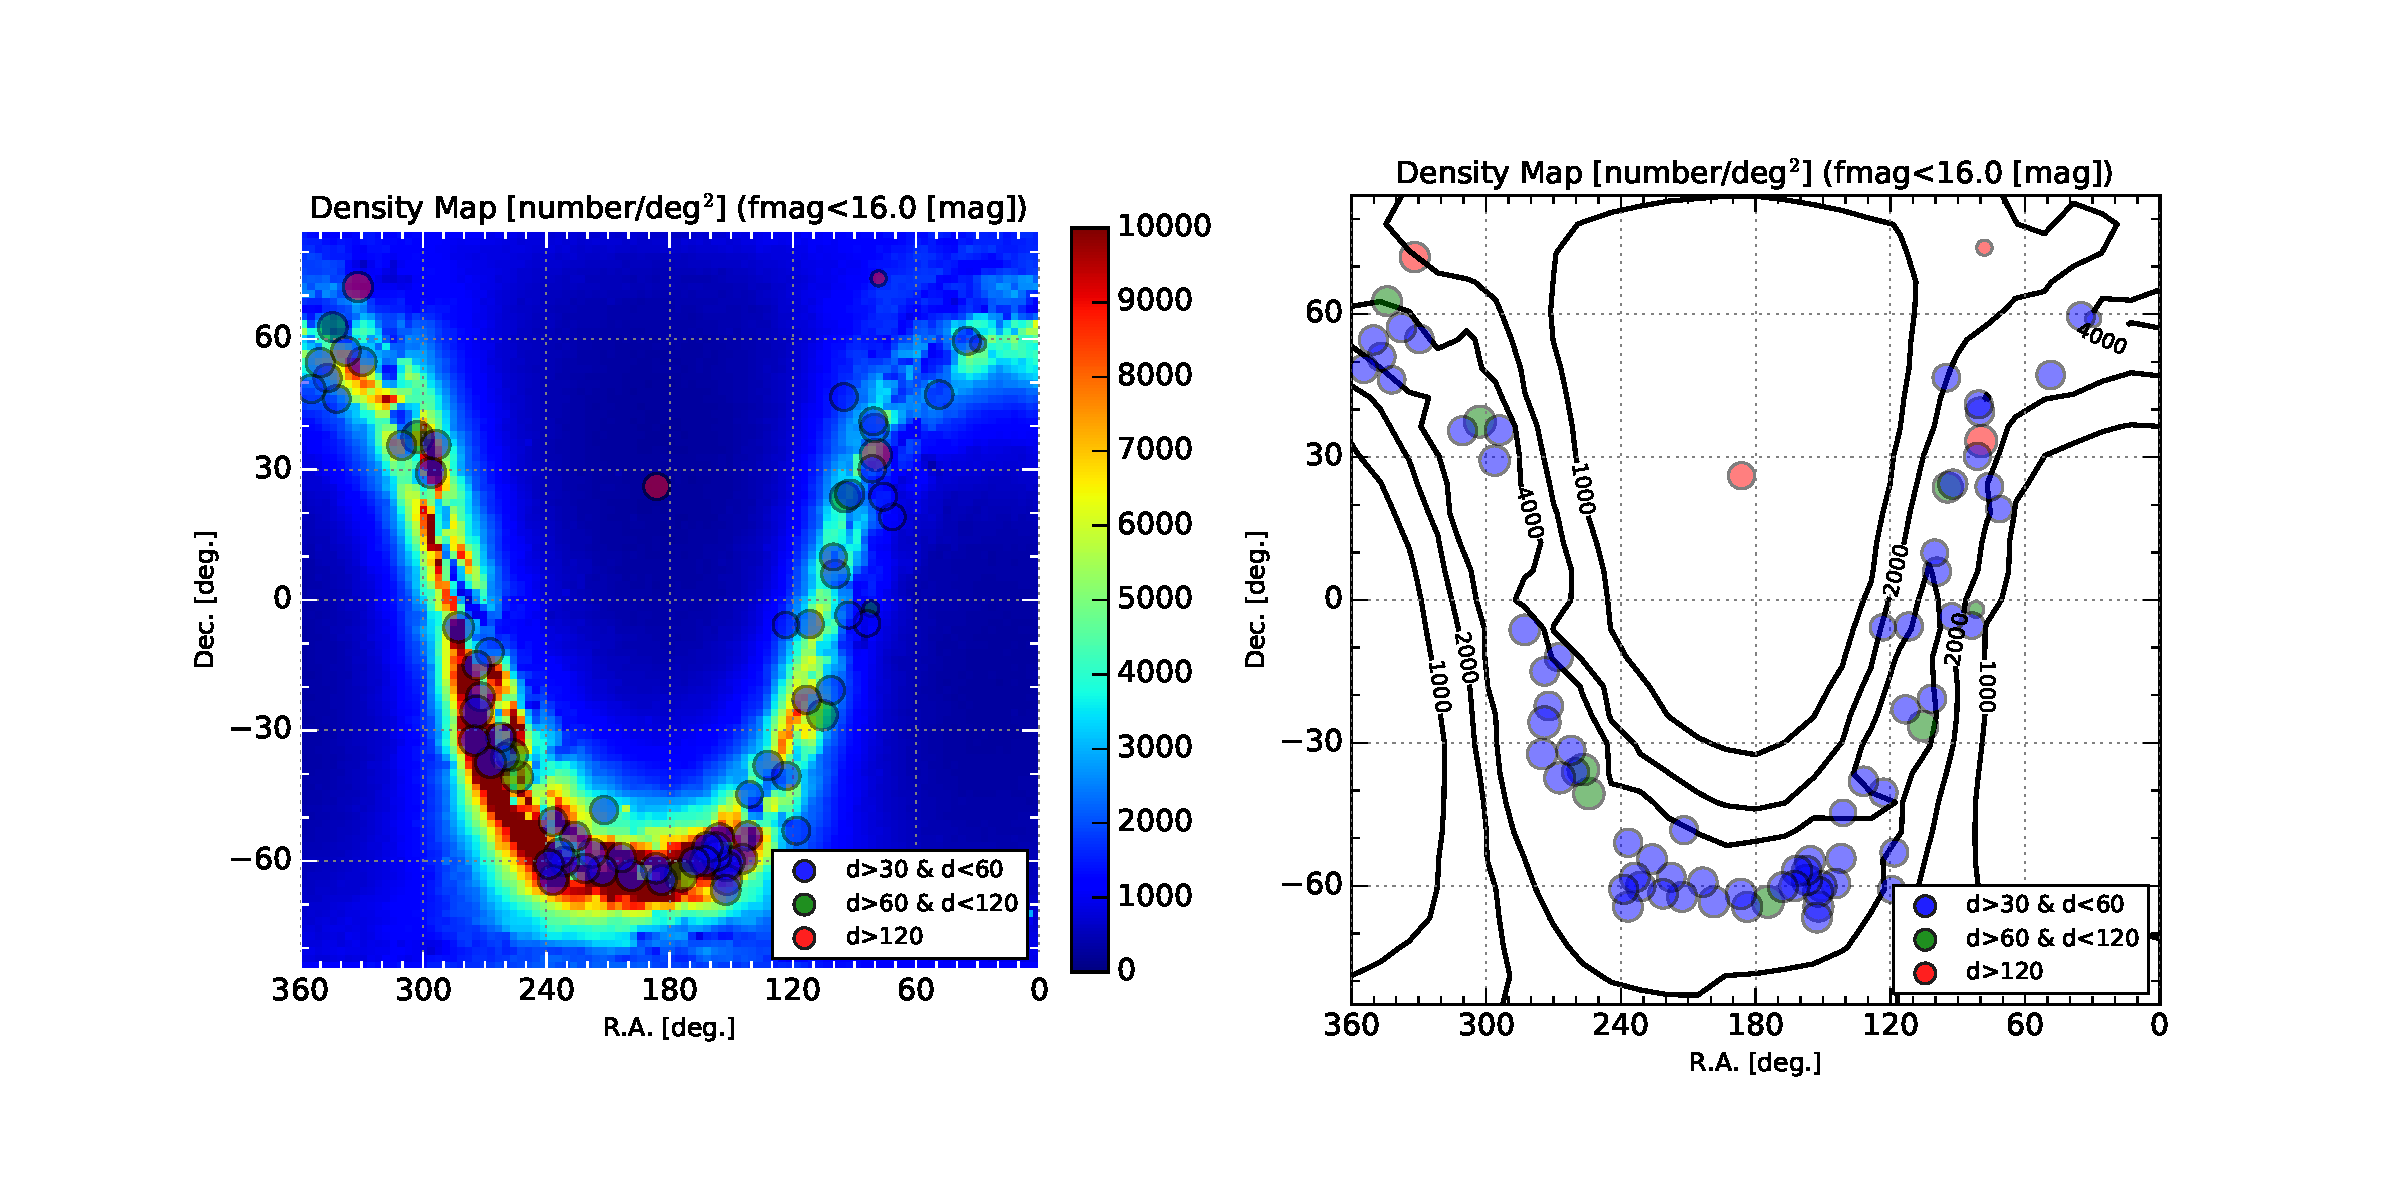
\includegraphics[width=150mm]{map_ucac4_openclusters_combined_f160.pdf}
\end{center}
\caption{Stellar density with objects $f<16.0$ mag taken from UCAC4 catalog in color map (left) and contour (right). The spatial distribution of open clusters with the apparent diameter ($d$ [deg.]) of $d>30$. from DAML02 catalogue is also plotted in both panels. Open clusters with $30<d<60$, $60<d<120$, and $d>120$ are shown by \textit{blue}, \textit{green}, and \textit{red circles}, respectively. The size of symbols represents the number of member stars.
}
\label{fig:RasterFieldMap1}
\end{figure}

\begin{figure}[!ht]
\begin{center}
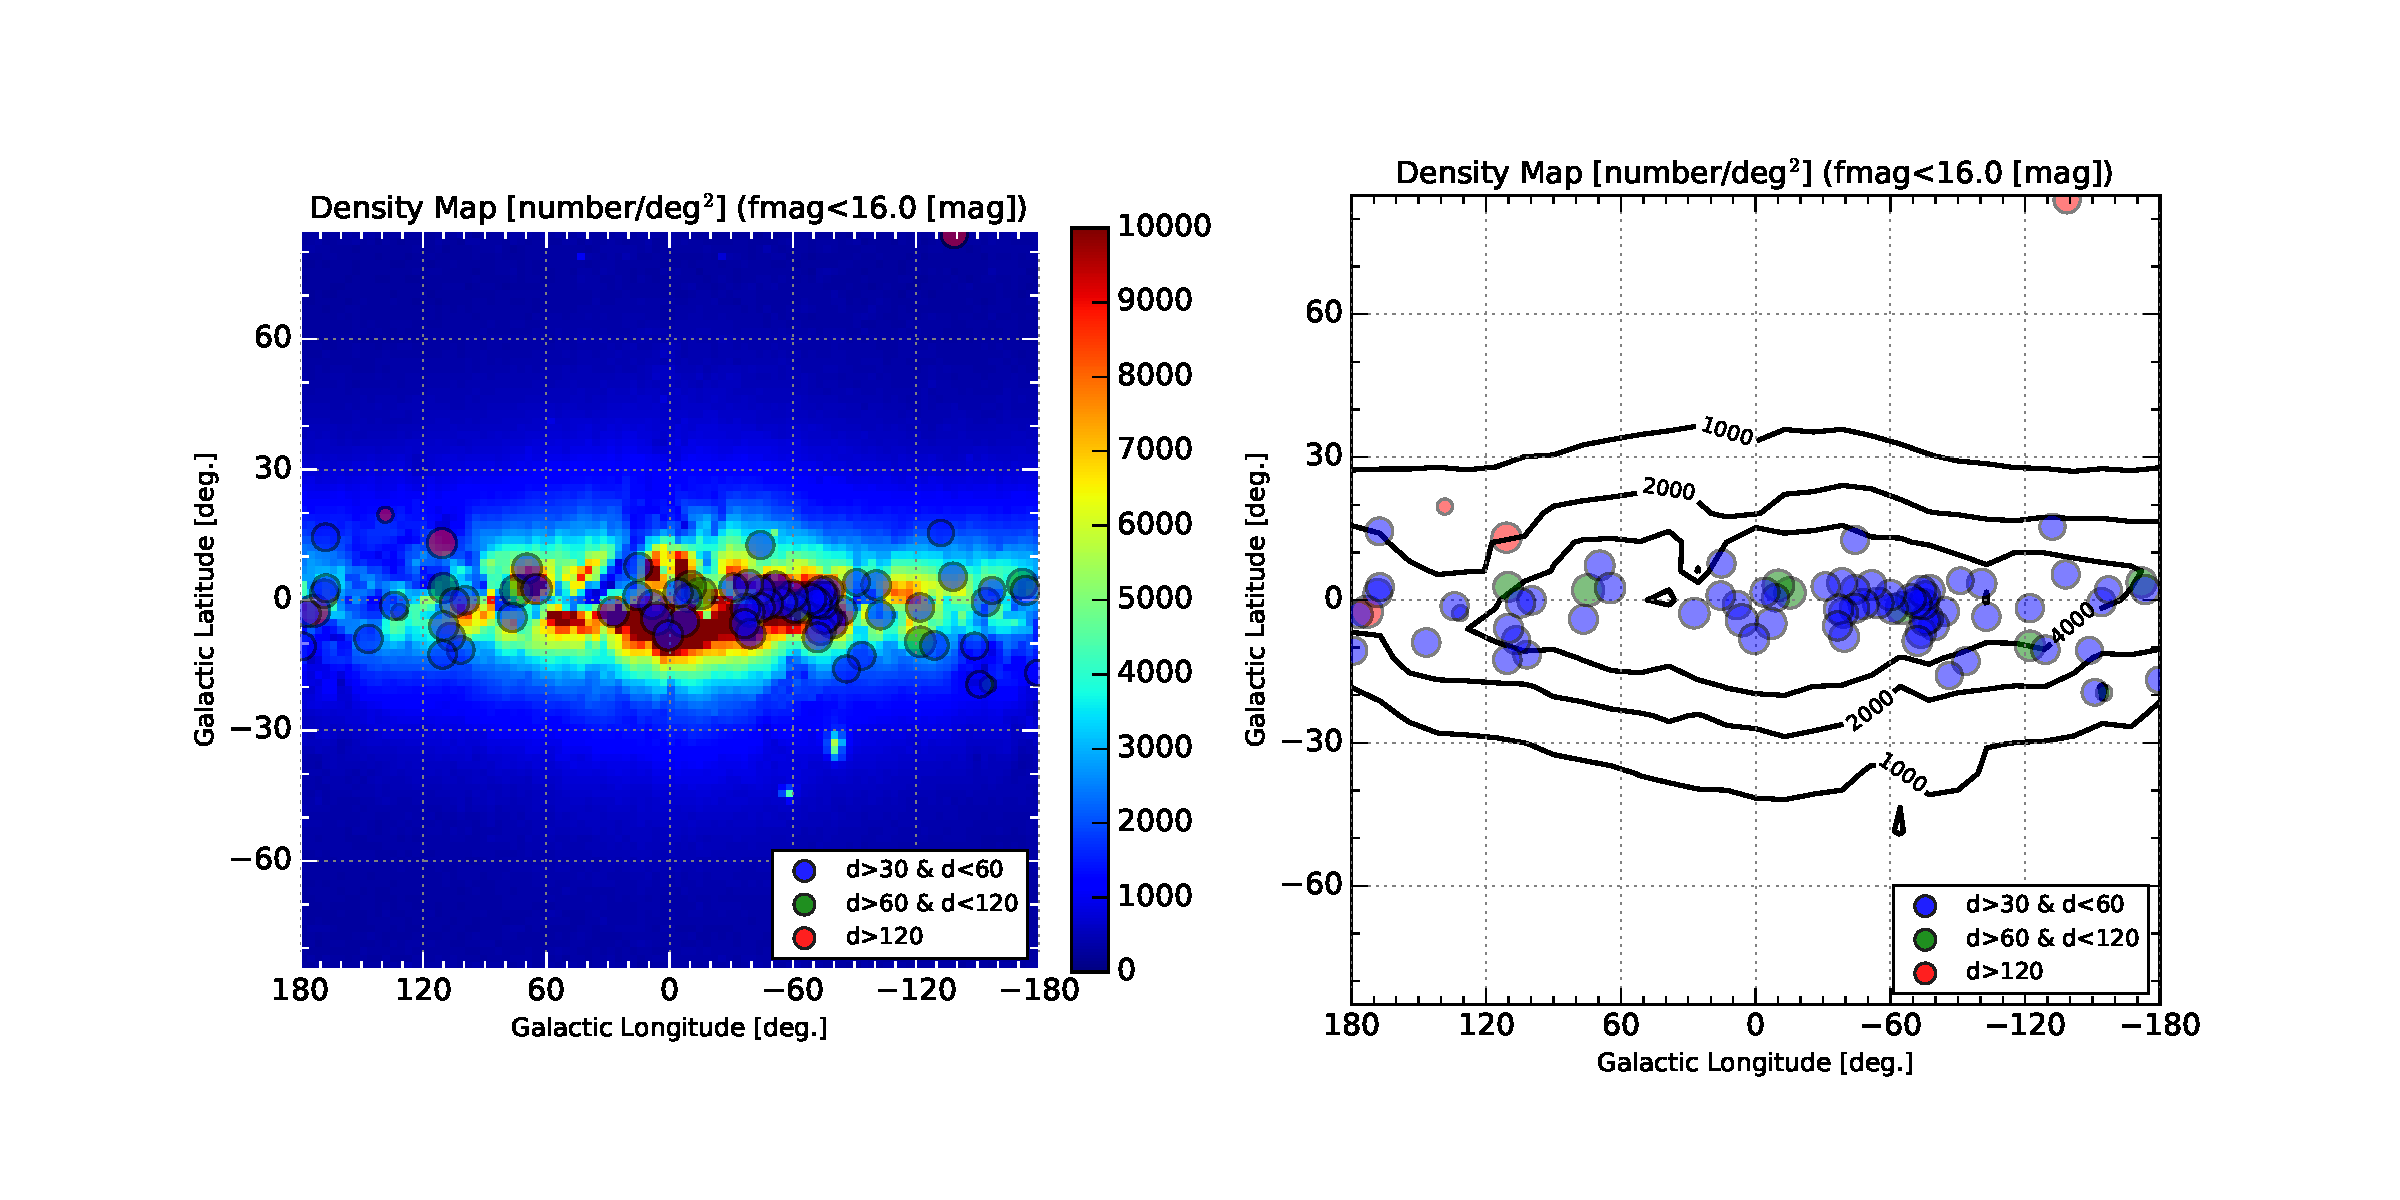
\includegraphics[width=150mm]{map_ucac4_openclusters_combined_f160_gc.pdf}
\end{center}
\caption{Similar to Figure \ref{fig:RasterFieldMap1}, but on the Galactic longitude and latitude.
}
\label{fig:RasterFieldMap2}
\end{figure}


\begin{table}[!ht]
\begin{center}
\caption{}
\label{tab:open_clusters}
\begin{tabular}{lccccc}  \hline
Name &  R.A. & Dec. & Diameter & \# of members & Mag. limit\\ 
          & [hh:mm:ss] & [dd:mm:ss] & [arcmin] & & [mag]\\
\hline \hline
Collinder 464 & 05:12:39 & +73:58:29  & 120.0 &  5212 & TBC  \\
Melotte 31     & 05:18:10 & +33:22:25  & 135.0  & 14341 & TBC \\
Melotte 111   & 12:25:06  & +26:06:00 & 120.0   & 863 & TBC    \\         
Collinder 471 & 22:07:06  & +72:00:00 & 130.0  & 4573 & TBC \\
\hline
ASCC 19       & 05:27:47 & $-$01:58:48  &  96.0    &  2412 & TBC \\
Collinder 89   & 06:18:00 & +23:38:00  &  60.0    &  2971 & TBC \\
Alessi 33        & 07:01:59 & $-$26:30:12  &  60.0   &   3371 & TBC \\
IC 2944$^{*}$  & 11:38:20  & $-$63:22:22  &  65.0   &  8860 & TBC \\
Trumpler 24$^{*}$  & 16:57:00  & $-$40:40:00 &  60.0   &  5720 & TBC \\
ASCC 88$^{*}$    & 17:06:47  & $-$35:36:00  &  66.0  &  6501 & TBC \\
ASCC 111       &  20:11:13 & +37:27:00 &  66.0  &  8004 & TBC \\
ASCC 125      &  22:56:17 & +62:45:00  &  66.0  &  2332 & TBC \\
\hline \hline
\end{tabular}
\end{center}
*: These targets cannot be observed with a good visibility.
\end{table}


\subsection{Field Bright Stars}
As Figure \ref{fig:RasterFieldMap1} and Figure \ref{fig:RasterFieldMap2} show, the spatial location of the available open clusters with sufficient apparent diameter for the PFS FoV is very limited. We thus consider the possibility of using normal field stars as raster scan targets in this subsection. In Figure \ref{fig:RasterFieldMap1} and Figure \ref{fig:RasterFieldMap2}, the density map of stars with $f<16.0$ mag. selected from the UCAC4 catalogue (Zacharias et al. 2013, AJ, 145, 44), which contains 113 million stars down to $R\sim16$ mag for which the positions determined with the accuracy of $<100$ mas. Although the number of available stars in one PFS FoV is limited in the high galactic latitude ($b$), there exist sufficient available stars of f$<16$ mag in $b<60$ deg.

\subsection{Faint Galaxies and Stars}
Basically, faint targets to verify the system performance will be selected from objects detected with HSC imaging data, which are candidate targets in the actual large survey with PFS. 
Inputs from 1D-DRP are appreciated as training/test set.

\subsection{Detailed Procedure of Raster Scan}
TBW

\subsection{List of Candidate Raster Fields}
TBW

\begin{figure}[!ht]
\begin{center}
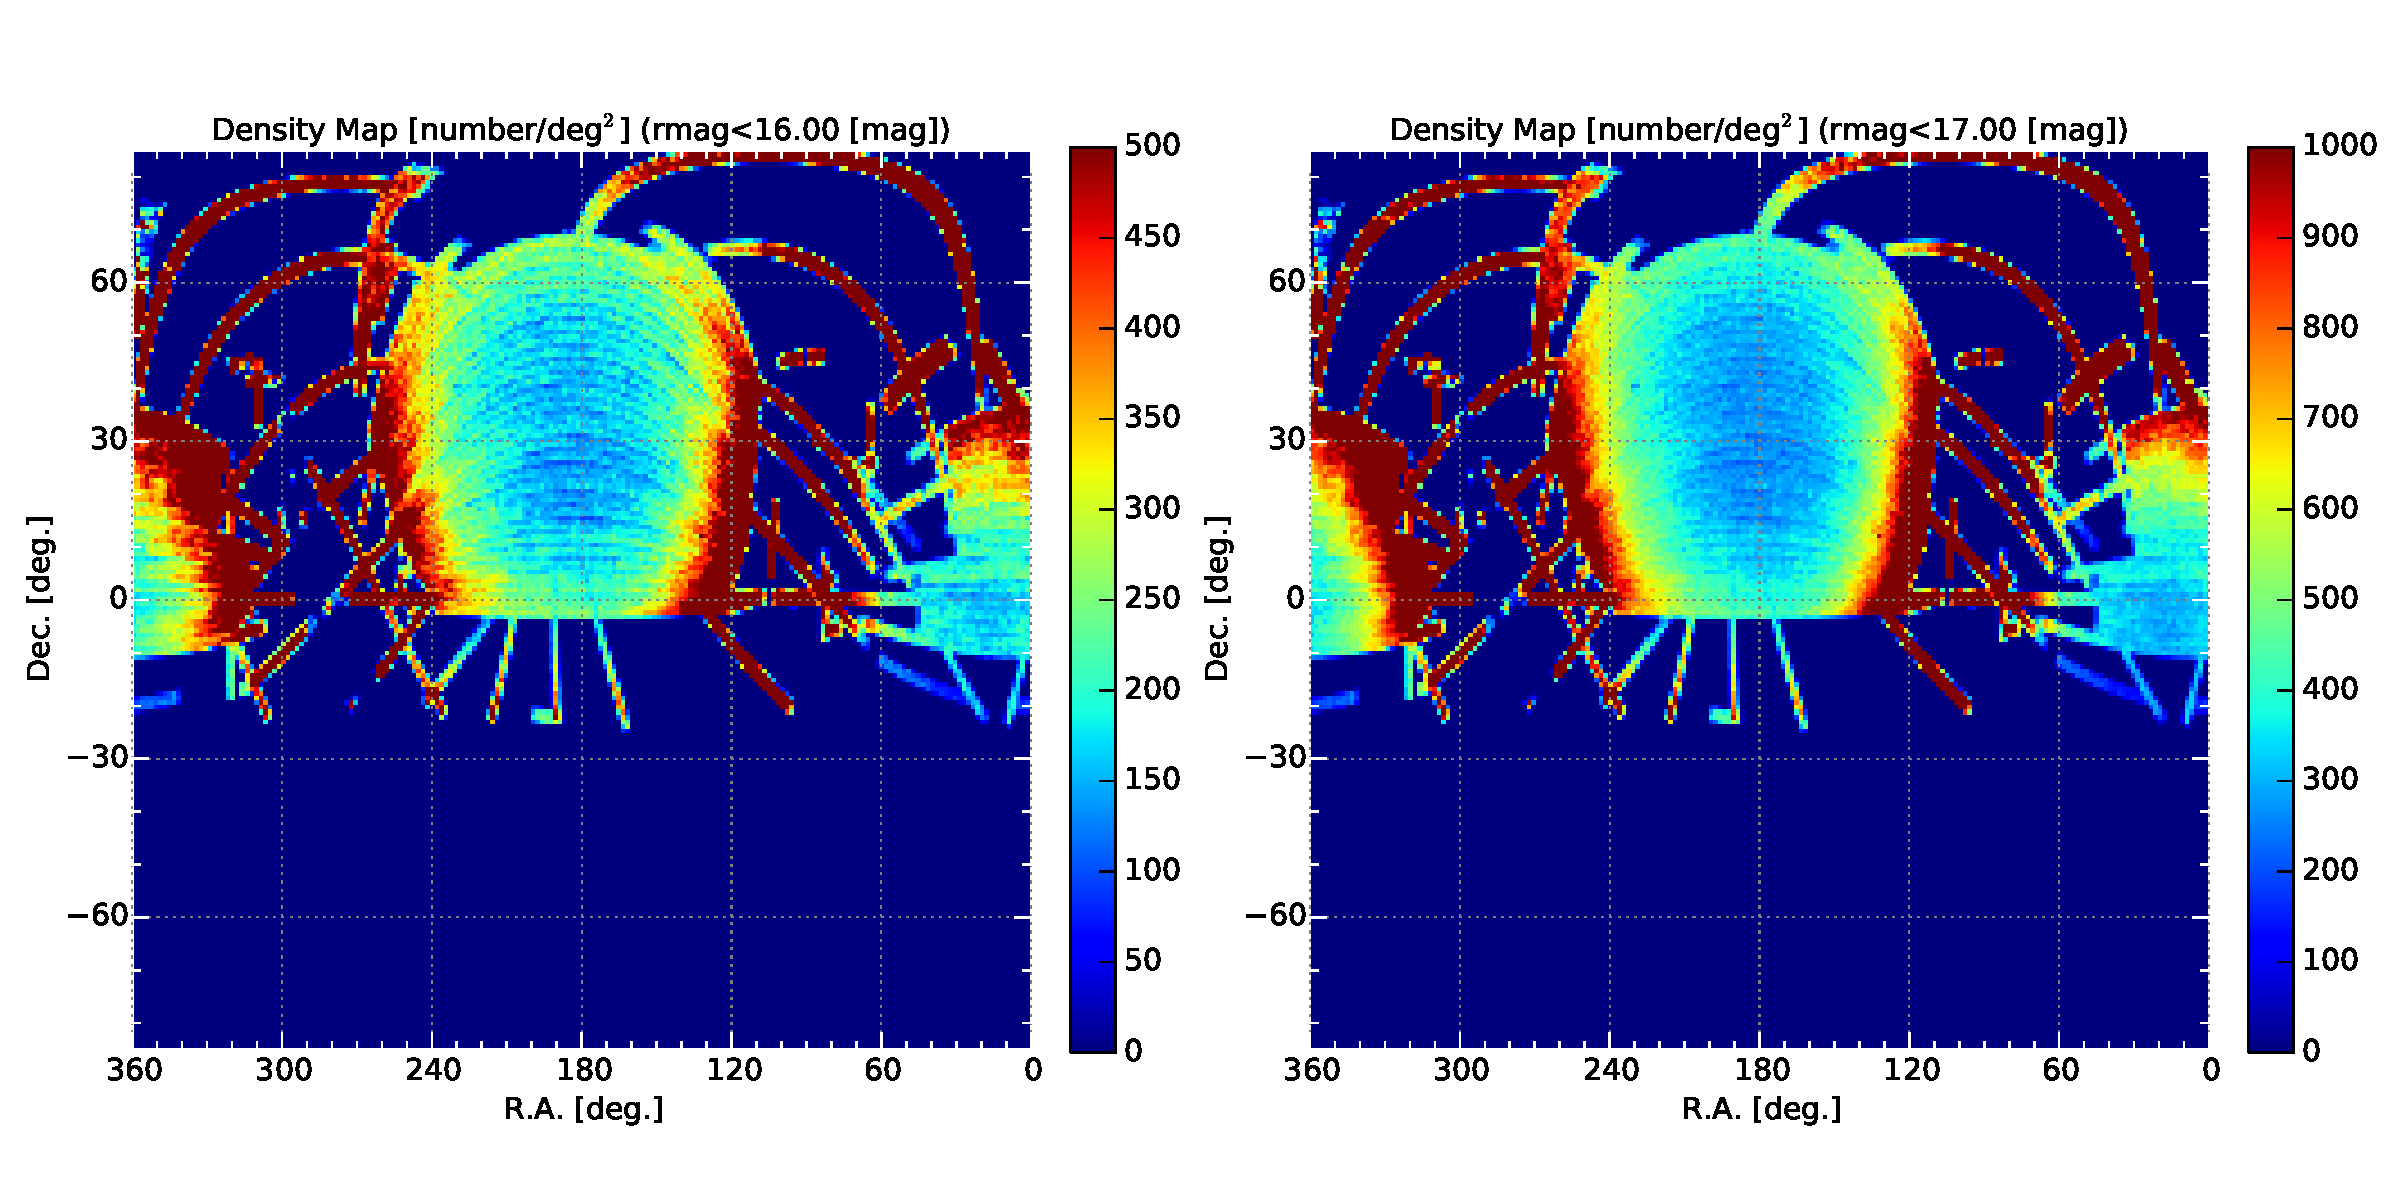
\includegraphics[width=150mm]{map_sdss_r16-17_colm_combined_20151208.pdf}
\end{center}
\caption{Stellar density with objects $r<16.0$ mag (left) and $r<17.0$ mag taken from SDSS DR12 catalog in color map. 
}
\label{fig:RasterFieldMapSDSS1}
\end{figure}

\begin{figure}[!ht]
\begin{center}
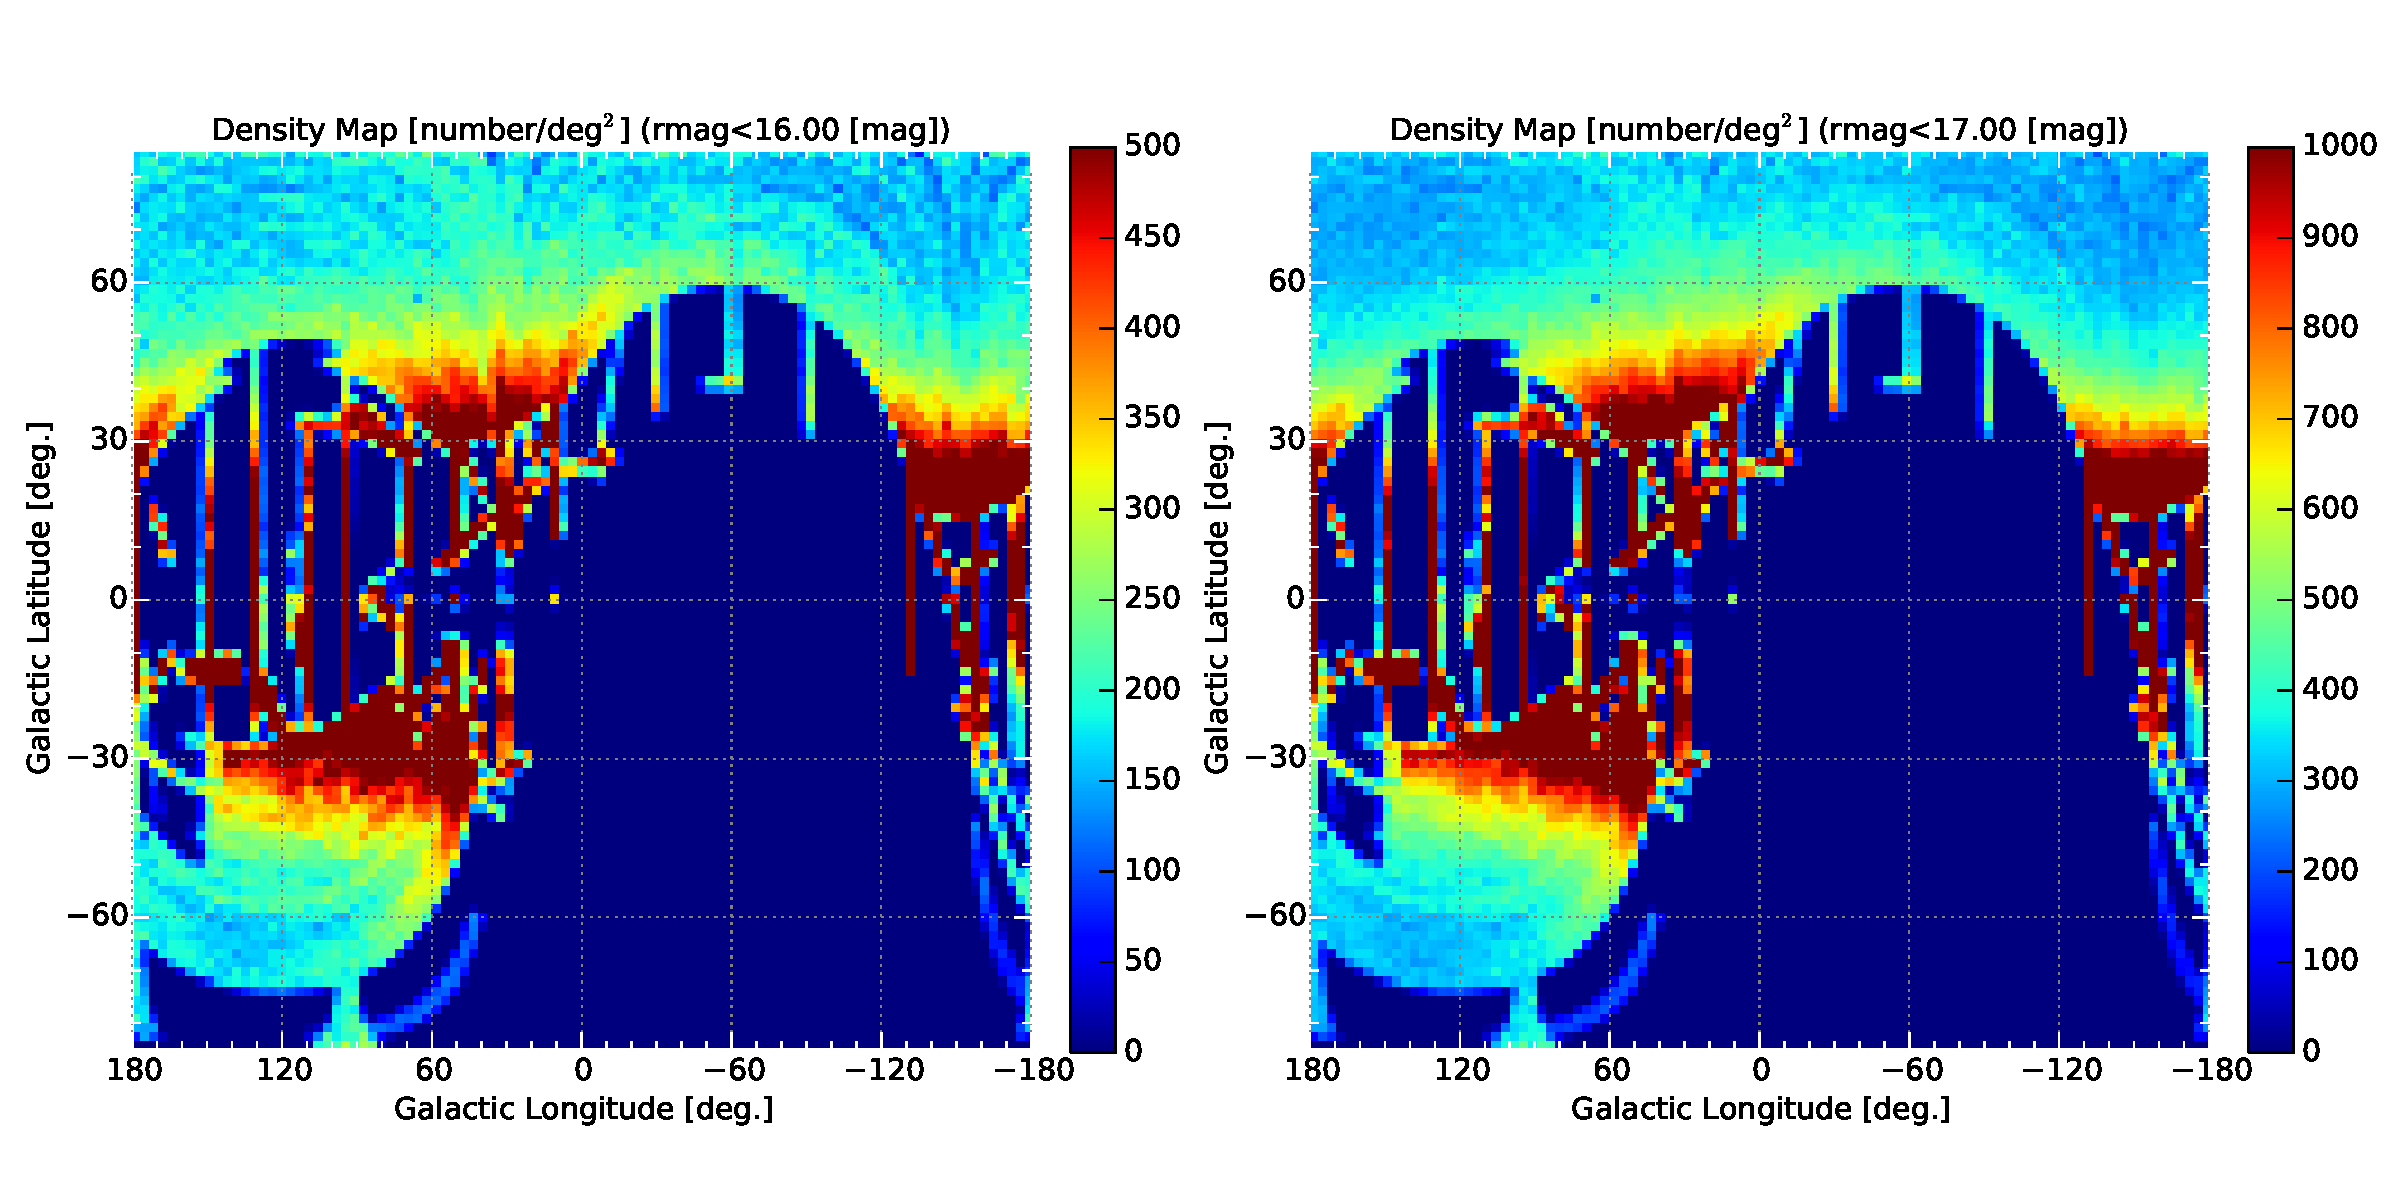
\includegraphics[width=150mm]{map_sdss_r16-17_colm_gc_combined_20151208.pdf}
\end{center}
\caption{Similar to Figure \ref{fig:RasterFieldMapSDSS1}, but on the Galactic longitude and latitude.
}
\label{fig:RasterFieldMapSDSS2}
\end{figure}


\subsection{List of Standard Star Catalogue}

TBW:
The data of the following standard stars are necessary for DRP/GA team:
\begin{itemize}
    \item Flux standard stars
    \item Radial velocity standard stars
    \item Telluric line standard stars
    \item Abundance standard stars
    \item $\log g$ standards stars
\end{itemize}
